\documentclass[border=10pt]{standalone}
\usepackage{tikz}

\begin{document}

    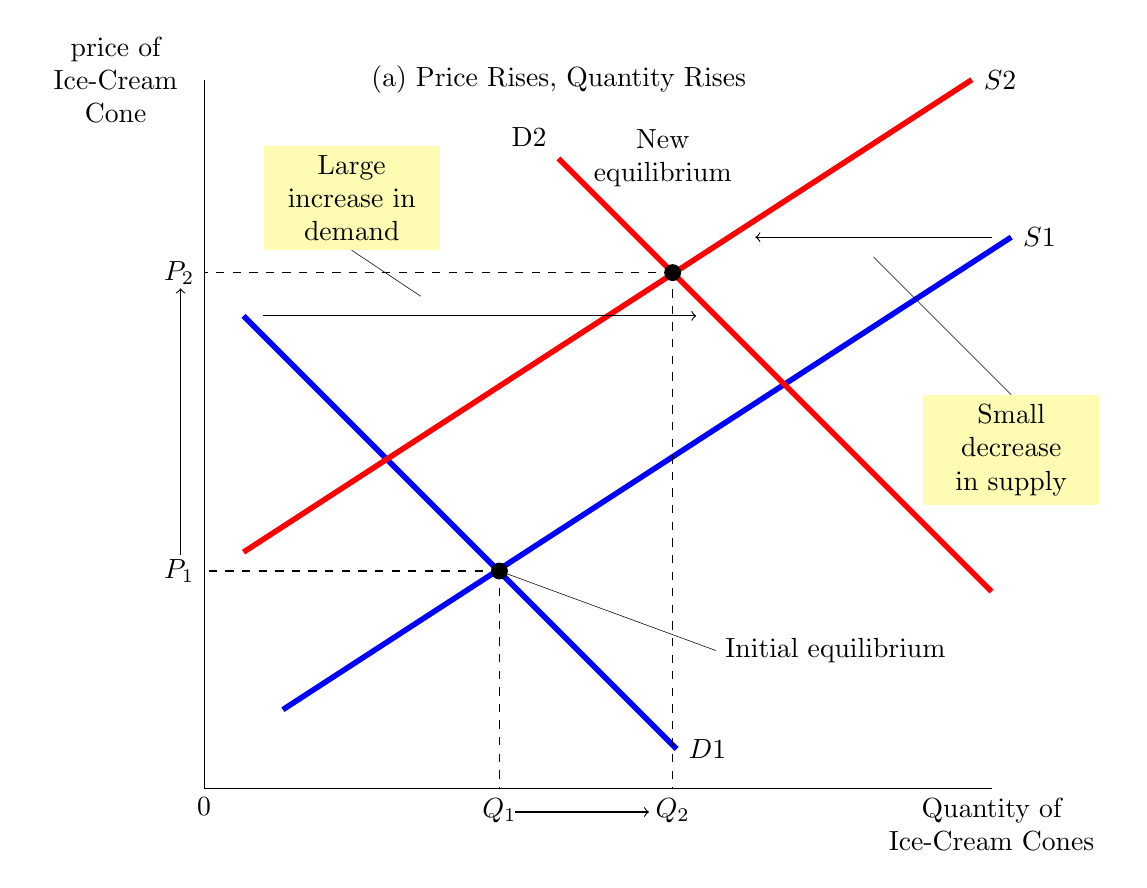
\begin{tikzpicture}

        \coordinate (O) at (0,0);
        \coordinate (a) at (1,1);
        \coordinate (b) at (0.5,6);
        \coordinate (s1) at (10.25,7);
        \coordinate (d1) at (6,0.5);
        \coordinate (q1) at (3.75,2.76);
        \coordinate (q2) at (5.95,6.55);
        \coordinate(c) at ([xshift=-0.5cm, yshift=2cm]a);
        \coordinate(d2) at ([xshift=4cm,yshift=2cm]d1);
        \coordinate(s2) at ([xshift=-0.5cm, yshift=2cm]s1);
        \coordinate(e) at ([xshift=4cm, yshift=2cm]b);
        \coordinate(f) at (q1|-O);
        \coordinate(g) at (q2|-O);
        \coordinate(h) at (O|-q1);
        \coordinate(i) at (q2-|O);
        


        \draw (O)--(10,0) node[below, text width=3cm, align=center]{Quantity of Ice-Cream Cones};
        \draw (O)--(0,9) node[left, text width= 2cm, align=center]{price of Ice-Cream Cone};
        \node[below](O){0};
        \draw[line width=2pt, blue] (b)--(d1) node[right, black]{$D1$};
        \draw[line width=2pt, blue] (a)--(s1) node[right, black]{$S1$};
        \draw[line width=2pt, red] (c)--(s2) node[right, black]{$S2$};
        \draw[line width=2pt, red] (d2)--(e) node[anchor=south east, black]{D2};
        \node[right] at (2,9) {(a) Price Rises, Quantity Rises};
        \draw[dashed](q1)--(f) node[below] {$Q_1$};
        \draw[dashed](q2)--(g) node[below]{$Q_2$};
        \draw[dashed](q1)--(h) node[left]{$P_1$};
        \draw[dashed](q2)--(i) node[left]{$P_2$};
        \draw[fill=black] (q1) circle[radius=1mm];
        \draw[very thin] (q1)--(6.5,1.75) node[right]{Initial equilibrium};
        \draw[fill=black] (q2) circle[radius=1mm];
        \node[right, align=center, text width=2cm] at(4.7,8){New equilibrium};
        \draw[->] (0.75,6)--(6.25,6);
        \draw[->] (10,7)--(7,7);
        \node[right, fill=yellow!30, text width=2cm, align=center] (etiquette1) at (0.75,7.5){Large increase in demand};
        \node[below, text width=2cm, align=center, fill=yellow!30] (etiquette2) at (10.25, 5){Small decrease in supply};
        \draw[very thin] (etiquette1.south)--(2.75,6.25);
        \draw[very thin] (etiquette2.north)--(8.5,6.75);
        \draw[->] ([xshift=-0.3cm,yshift=0.2cm]h)--([xshift=-0.3cm,yshift=-0.2cm]i);
        \draw[->] ([xshift=0.2cm,yshift=-0.3cm]f)--([xshift=-0.3cm,yshift=-0.3cm]g);

        
    \end{tikzpicture}

    
\end{document}
